\subsection{相关性基础}


\subsubsection{1. 基本概念}


\begin{itemize}
\item Static financial correlations: measure how two or more financial assets are associated within a certain time period.
\end{itemize}

\begin{itemize}
\item Dynamic financial correlations: measure how two or more financial assets move together in time.
\end{itemize}

\begin{itemize}
\item Financial correlation risk: the risk of financial loss due to adverse movements in correlation between two or more variables. 【由于相关性不利变动而导致的损失风险。】
\end{itemize}


\begin{example}{例子}
    例子: An investor has invested \(\$ 1\) million in a bond from Spain， and purchased a CDS from a French bank， BNP Paribas， because he is now worried about Spain defaulting.【投资者投资了 100 万美元购买了一只西班牙债券， 因为他担心西班牙债券会违约， 从一家法国银行 BNP Paribas 购买了信用违约掉期(CDS)】
\end{example}




CDS 知识补充:

\hspace*{1em} 一个投资者 \(\mathrm{A}\) 买了一个 \(\mathrm{C}\) 公司发行的债券，但是担心 \(\mathrm{C}\) 公司未来违约

(信用风险)， 然后向一家 B 金融机构购买了一个"保险"， 提供的保护就是关

于公司 C 是否违约。

\checkmark 零时刻或者每期期初:投资者 A 向金融机构 B 支付保费(CDS spread)

\checkmark 未来:如果公司 C 违约

\checkmark 这里的"保险"就是我们将要介绍的 CDS

\checkmark 角色:

\hspace*{1em} 投资者 A: An investor

\hspace*{1em} 金融机构 B: BNP Paribas

\hspace*{1em} C 公司发行的债券: Spain bond



 我们这里关注的是西班牙债券和 BNP Paribas 违约相关性与 CDS spread 的关系。

\begin{center}
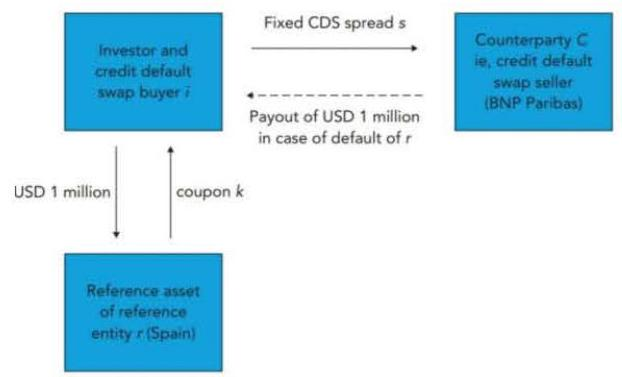
\includegraphics[width=0.5\textwidth]{images/spread.jpg}
\end{center}
\hspace*{3em} 

\begin{itemize}
\item If the correlation between Spain and BNP Paribas increases， the value of the CDS will decrease and the investor will suffer a paper loss(账面损失)。
\end{itemize}

理解: Spain 债券违约了， 需要赔付， 结果你 BNP Paribas 也违约了， 那么我投资者就没有得到任何保护， 因此， 如果我预测他俩的违约相关性是比较高的， 我不会买 CDS 或者只愿意支付一个比较低的 CDS spread。

投资者希望两者的违约相关性越低，越好。

If there is a positive default correlation between the two， the investor has wrong-way correlation risk (WWR， 错路风险). 【如果这两者的违约相关性是正的， 投资者面临的风险叫作错路风险】

CDS spreads of a hedged bond purchase with respect to the default correlation between the Spain bond and the BNP Paribas.

\begin{center}
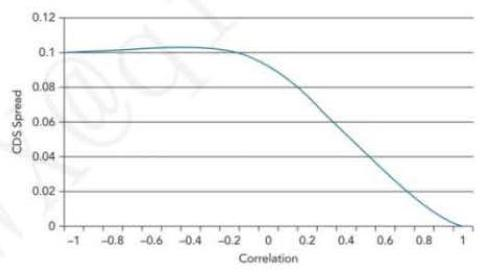
\includegraphics[width=0.4\textwidth]{images/correlation.jpg}
\end{center}
\hspace*{3em} 


\subsubsection{2. Correlations and correlation risk are everywhere in finance}


【原版书这里从 5 个方面进行介绍， 有的比较简单， 是咱们 FRM 一直学习的理念。】

\begin{itemize}
\item Investment
\end{itemize}

\begin{itemize}
\item Trading
\end{itemize}

\begin{itemize}
\item Risk management
\end{itemize}

\begin{itemize}
\item The global financial crisis
\end{itemize}

\begin{itemize}
\item Regulation
\end{itemize}

 监管 Regulation 与相关性:相关性在监管框架中扮演关键角色，尤其在巴塞尔协议中， 针对市场风险和信用风险方面的规定。

关于这个知识主要出现在《操作风险》这个科目中，这里不做介绍(原版书这里也没有做详细介绍)。

(1) Investments and Correlation

\begin{itemize}
\item 两资产构成的组合， 其收益和标准差:
\end{itemize}

\[
{R}_{p} = {w}_{1}{R}_{1} + {w}_{2}{R}_{2}
\]

\[
{\sigma }_{p} = \sqrt{{w}_{1}{}^{2}{\sigma }_{1}{}^{2} + {w}_{2}{}^{2}{\sigma }_{2}{}^{2} + 2{w}_{1}{w}_{2}{\rho }_{1，2}{\sigma }_{1}{\sigma }_{2}}
\]

The negative relationship of the portfolio return/ portfolio risk ratio with respect to the correlation of the assets in the portfolio。【相关性不影响 return， 只会影响 risk】

\begin{center}
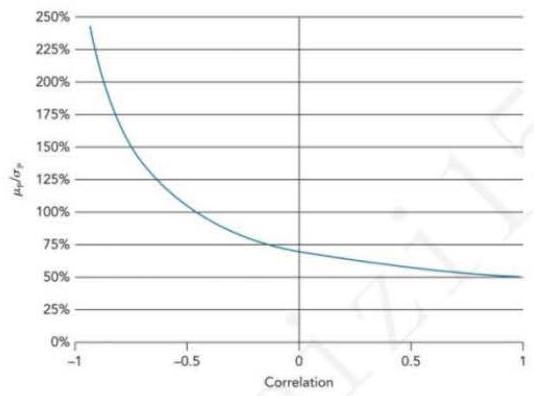
\includegraphics[width=0.4\textwidth]{images/crls.jpg}
\end{center}
\hspace*{3em} 

(2) Trading and Correlation

\begin{itemize}
\item Correlation trading means trading assets， whose price is determined at least in part by the co-movement of one asset or more in time.
\end{itemize}

A. Multi-asset options 多资产期权

\begin{itemize}
\item 也叫 rainbow options or mountain-range options.具体种类【具体每个期权混个脸熟】:
\end{itemize}

Options on the better of two:payoff \(= \operatorname{Max}\left( {{\mathrm{S}}_{1}，{\mathrm{\;S}}_{2}}\right)\)

Options on the worse of two: payoff = \(\operatorname{Min}\left( {{\mathrm{S}}_{1}，{\mathrm{\;S}}_{2}}\right)\)

Call on the Maximum of two: payoff = \(\max \left\lbrack  {0，\max \left( {{\mathrm{S}}_{1}，{\mathrm{\;S}}_{2}}\right)  - \mathrm{K}}\right\rbrack\)

Exchange option(such as a convertible bond): payoff = \(\max \left( {0，\mathrm{S}1 - \mathrm{S}2}\right)\)

Spread call option: payoff = \(\max \left\lbrack  {0，\left( {\mathrm{S}1 - \mathrm{S}2}\right)  - \mathrm{K}}\right\rbrack\)

Option on the better of two or cash: Payoff \(= \max \left( {\mathrm{S}1，\mathrm{\;S}2，\text{ cash }}\right)\) .

Dual strike call option: \(\operatorname{Payoff} = \max \left( {0，\mathrm{S}1 - \mathrm{K}1，\mathrm{\;S}2 - \mathrm{K}2}\right)\) .

Basket option: \(\left\{  {n}_{i}\right.\) is the weight of assets \(i\)  payoff \(=\)

\[
\left\lbrack  {\mathop{\sum }\limits_{{i = 1}}^{n}{n}_{i}{s}_{i} - k，0}\right\rbrack
\]

\begin{itemize}
\item the price of these correlation options is highly sensitive to the correlation between the asset prices \({\mathrm{S}}_{1}\) and \({\mathrm{S}}_{2}\) .
\end{itemize}

B. Quanto options(双币种期权)

\begin{itemize}
\item Quanto options， options that allow a domestic investor to exchange his potential option payoff in a foreign currency back into his home currency at a fixed exchange rate. 【投资的标的是外国资产，但是以本币进行支付的， 比较担心汇率的变动】
\end{itemize}

\begin{itemize}
\item A quanto option therefore protects an investor against currency risk
\end{itemize}

 The correlation between the price of the underlying (S) and the exchange rate (X) significantly influences the quanto call option price 【标的资产价格(S)与汇率(X)之间的相关性， 影响 quanto call 的价格。】

\begin{itemize}
\item 原版书例子， an American believes the Nikkei will increase， but she is worried about a decreasing yen. The investor can buy a quanto call on the Nikkei， with the yen payoff being converted into dollars at a fixed exchange rate. 【一位美国投资者认为日经指数将上涨， 但她担心日元贬值。那么投资者可以购买 quanto call on the Nikkei， 其中日元将以固定汇率转换为美元。】
\end{itemize}

If the correlation is positive， an increasing Nikkei will also mean an increasing yen. That is favorable for the call seller. She has to settle the payoff， but only needs a small yen amount to achieve the dollar payment.

如果相关性比较大， 日经指数上涨也将意味着日元升值。quanto call 不会行权(如果行权，是以固定汇率将日元转为美元，反而不利)。 也就是对 quanto call 的 buyer 不利。那么 quanto call 的价格就不会高。

The more positive the correlation coefficient， the lower the price for the quanto option.

The lower the correlation coefficient， the more expensive the quanto option. 【也就是 quanto call 的购买者， 希望相关性越低越好， 买了这个期权， 才有用】

C. Correlation swap 相关性互换

\begin{itemize}
\item Correlation swap: a fixed (ie， known) correlation is exchanged with the correlation that will actually occur， called realised or stochastic (ie， unknown) correlation。
\end{itemize}

简言之，相关性互换就是固定的相关性和浮动的相关性交换。

\begin{itemize}
\item Paying a fixed rate in a correlation swap is also called "buying correlation".
\end{itemize}

理解:buying correlation，相关性上升赚钱。在相关性互换中，收浮动相关性， 才能在相关性上升时赚钱。收浮动相关性， 对应着支固定相关性。

\begin{itemize}
\item correlation swap (the correlation fixed rate Payer) payoff: 【这两个公式要掌握】
\end{itemize}

\[
\text{ payoff } = \mathrm{{NP}} \times  \left( {\text{ realized }\rho  - \text{ fixed }\rho }\right)
\]

\[
{\rho }_{\text{ realized }} = \frac{2}{{\mathrm{n}}^{2} - \mathrm{n}}\mathop{\sum }\limits_{{\mathrm{i} > \mathrm{j}}}{\rho }_{\mathrm{i}，\mathrm{j}}
\]

 NP: 合约规模

 \({\rho }_{i，j}\) : Pearson correlation between asset \(i\) and \(j\)

\begin{itemize}
\item n: number of assets
\end{itemize}

D. Another way of buying correlation (ie， benefiting from an increase in correlation) is to buy put options on an index such as the Dow Jones Industrial Average (Dow) and sell put options on individual stock of the Dow.

\section*{【购买某个指数 (如 Dow) 的看跌期权， 并卖出该指数成分股的看跌期权】}

\begin{itemize}
\item 背景:当市场下行时，相关系数上涨，指数的相关系数上涨幅度超过个股相关系数上涨幅度。
\end{itemize}

\begin{itemize}
\item If the correlation between the stocks of the Dow increases， for example in a market downturn， so will the implied volatility of the put on the Dow. 【相关性和波动率之间存在正向关系】
\end{itemize}

\begin{itemize}
\item This increase is expected to outperform the potential loss from the increase in the short put positions on the individual stocks.
\end{itemize}

\begin{itemize}
\item 该策略是通过指数看跌期权的涨幅超过 individual stock 看跌期权的潜在损失。整体策略是赚钱的。
\end{itemize}

\begin{itemize}
\item 2012 年， London whale 伦敦鲸案例， JP Morgan 出现大量损失， 就是由于这种策略: sold CDSs on an index of bonds， the CDX.NA.IG.9， and "hedged" it with buying CDSs on individual bonds.
\end{itemize}

(3) Risk Management and Correlation

\begin{itemize}
\item Correlation Risk and Market Risk
\end{itemize}

通常使用 VaR 来衡量市场风险， VaR 隐含地包含了相关性风险

 Correlation risk is an integral part of market risk.

\[
{Va}{R}_{p} = \sqrt{x}{\sigma }_{p}\alpha
\]

 \({\sigma }_{\mathrm{p}}\) : the daily volatility of the portfolio， including the correlation among the assets.

 \(\alpha\) :the z-value from the standard normal distribution for a specific confidence level. 【就是 Z 值】

 \(\mathrm{x}\) : the number of trading days.

The VaR for the portfolio increases as the correlation among the assets in the portfolio increases.

\begin{center}
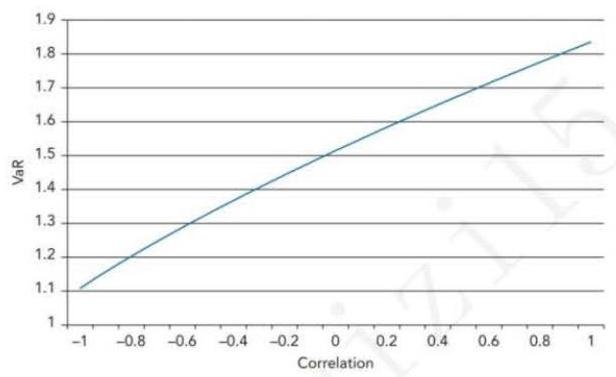
\includegraphics[width=0.5\textwidth]{images/crlss.jpg}
\end{center}
\hspace*{3em} 

\begin{itemize}
\item Correlation Risk and Credit Risk
\end{itemize}

\begin{itemize}
\item According to the historical data， we observe that the default correlation within sectors is higher than between sectors. 【行业内的违约相关性高于行业间的相关性】
\end{itemize}

This suggests that macro systematic factors have a greater impact on defaults than do idiosyncratic factors.

For most investment grade bonds， the term structure of default probabilities increases in time. 【对于大多数投资级债券， 违约概率的期限结构随着时间的推移而增加。比如下图中评级 A 的债券。】

解释原因: The longer the time horizon， the higher the probability of adverse internal events.

For bonds in distress， the term structure of default probabilities decreases in time. 【比如下图中评级 CC 的债券。】

解释原因: For a distressed company the immediate future is critical. If the company survives the coming problematic years， probability of default decreases. 【对于处于困境的公司，如果能挺过当前比较糟糕的情况， 未来变好的可能性更大】

\begin{center}
\adjustbox{max width=\textwidth}{
\begin{tabular}{|c|c|c|c|c|c|c|c|c|c|c|}
\hline
Year & \phantom{X} & \phantom{X} & \phantom{X} & \phantom{X} & \phantom{X} & \phantom{X} & \phantom{X} & \phantom{X} & \phantom{X} & \phantom{X} \\
\cline{1-11}
\phantom{X} & 1 & 2 & 3 & 4 & 5 & 6 & 7 & 8 & 9 & 10 \\
\cline{1-11}
A & 0.02\% & 0.07\% & 0.13\% & 0.14\% & 0.15\% & 0.17\% & 0.18\% & 0.21\% & 0.24\% & 0.25\% \\
\cline{1-11}
CC & 23.83\% & 13.29\% & 10.31\% & 7.62\% & 5.04\% & 5.13\% & 4.04\% & 4.62\% & 2.62\% & 2.04\% \\
\cline{1-11}
\hline
\end{tabular}
}
\end{center}

Term Structure of Default Probabilities for an A-rated Bond and a CC-Rated Bond in 2002

\begin{itemize}
\item Correlation risk and systemic risk
\end{itemize}

 Systemic risk: the risk of a financial market or an entire financial system collapsing.

A Systemic risk and correlation risk are highly dependent.

A systemic decline in stocks involves the entire stock market， correlations between the stocks increase sharply. 【股票市场的系统性下跌会涉及整个股票市场， 股票之间的相关性急剧增加。】

Correlation risk and concentration risk

\begin{itemize}
\item Concentration risk 集中度风险: the risk of financial loss due to a concentrated exposure to a group of counterparties.
\end{itemize}

\begin{itemize}
\item Concentration risk can be quantified with concentration ratio 集中度比率.
\end{itemize}

E.g.， if creditor has 10 loans of equal size， the concentration ratio is 0.1 .

The lower the concentration ratio， the more diversified is the default risk of the creditor.

\begin{itemize}
\item In particular， both a lower concentration ratio and a lower correlation coefficient reduce the worst-case scenario for a creditor， the joint probability of default of his debtors. 【较低的集中度比率和较低的相关系数都降低了债权人的 worst-case scenario， 即其债务人违约的联合概率。】
\end{itemize}

\section*{(4) The Global Financial Crises and Correlation}

\begin{itemize}
\item 这里主要关注的是 2007 年到 2009 年全球危机和相关性的关系。在这次全球金融危机中，相关性在很大程度上加剧了危机的爆发和扩大:【原版书这里给的内容较多， 这里可以重点关注 CDO 这里】
\end{itemize}

A. 低估了违约风险:2003 年至 2006 年期间，金融市场处于极其宽松的环境。在这种环境下， 普遍低估了违约风险， 并大量借贷投资于房地产、 金融市场等各个领域，导致了各个市场出现了泡沫。

B. 结构化产品的崛起: 新型结构化产品，如 CDOs、CDO squared 等产品的出现。这些结构化产品往往依赖于不同资产之间的相关性。

 以 CDO 为例，展示相关性在结构化产品中的作用。

\begin{center}
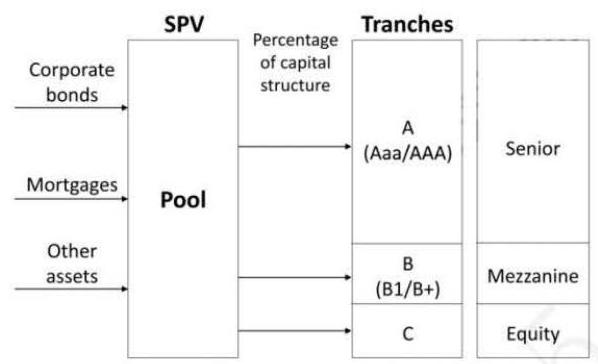
\includegraphics[width=0.5\textwidth]{images/SPV.jpg}
\end{center}
\hspace*{3em} 

知识简介:CDO 一般会有各种层级 (tranche)。典型的分为:高级层 (senior tranche)、夹层 (mezzanine tranche) 及股权层 (equity tranche) 。senior 层的风险最小， 收益也最小， equity 层的风险最大， 收益也最大。如果有损失， 首先由 equity 层承担， 然后 mezzanine 层承担， 最后 senior 层承担。

From 2007 to 2009， default correlations of the mortgages in the CDOs increased. This actually helped equity tranche investors.

 If default correlations increase， the equity tranche spread decreases， leading to an increase in the value of the equity tranche.

 解释: 前提违约概率不变。

 当default correlations 非常高， 比如假设违约相关性是 1 ， 意味着这些贷款要么全部违约，要么全部不违约。如果全部违约，此时 senior 、 mezzanine 及 equity 都有损失。如果全部不违约， 此时 senior、 mezzanine 及 equity 都能收到投资现金流。所以， 三个层级风险相同， 但是 equity 未来的收益更大， 更受市场欢迎。所以 increase in the value of the equity tranche。那么针对 equity tranche 的保险， 其保费 spread 也更低。

 当default correlations 非常低， 比如假设违约相关性是-1。意味着这些 mortgages 有人违约， 有人不违约。如果发生了违约， 那么 equity 层会承担这些损失。那么相对的， mezzanine 安全一点， senior 最安全。所以， 如果预计违约相关性比较低时， equity 的价值是下降的。】

However， this increase was overcompensated by a strong increase in default probability of the mortgages. 【这句话的意思是， 如果违约概率上升， 违约相关性是怎么样的就显得不那么重要了。即如果 strong increase in default probability， 所有的贷款都会违约， 所有的 tranche 都会违约，都会"死"掉。这正是这次危机的情况】

As a consequence， tranche spreads increased sharply， resulting in huge losses for the equity tranche investors as well as investors in the other tranches.

What is more， correlations between the tranches of the CDOs also increased during the crisis.

C. 相关性模型的误导: 新型 copula 相关性模型被投资者误以为是能够准确度量资产之间的相关性， 而实际上这些模型在极端情况下的预测能力存在很大的缺陷。

D. 信用评级机构的道德风险 moral hazard : 信用评级机构受到支付评级费用的公司的影响， 可能会给予比较高的评级， 使得结构化产品看起来风险较低。

E. 投资者的过度投机。

\subsubsection{相关性和相关性风险在金融领域无处不在 }


\subsection{相关性的经验性质}


这一节的内容，主要是一些实证结论。 (1) Equity correlations and correlation volatilities

\begin{itemize}
\item The worse the state of the economy the higher are equity correlations.
\end{itemize}

Equity correlations were extremely high during the great recession of 2007-09 and reached 96.97\% in February 2009. 【经济状况越糟糕，股票之间的相关性就越高。2007 年至 2009 年的大衰退期间，股票相关性极高，2009 年 2 月达到了 96.97\%。】

\begin{itemize}
\item Equity correlation volatility is lowest in an expansionary period and higher in normal and recessionary economic periods. 【在扩张期， 股票相关性的波动性最低，在正常和衰退经济期间较高。】
\end{itemize}

\begin{itemize}
\item Equity correlation levels and equity correlation volatility are positively related.
\end{itemize}

\begin{itemize}
\item 债券相关性和股票相关性的关系: Bond correlation levels and bond correlation volatilities are generally higher in economic bad times. In addition， bond correlations exhibit mean reversion， although lower mean reversion than equity correlations exhibit.
\end{itemize}

\begin{itemize}
\item 违约相关性和股票相关性的关系: Default correlations also exhibit properties seen in equity correlations. Default probability correlation levels are slightly lower than equity correlation levels， and default probability correlation volatilities are slightly higher than equity correlations.
\end{itemize}

(2)mean reversion 均值复归和 Autocorrelation 自相关性

\begin{itemize}
\item mean reversion(均值复归):
\end{itemize}

\begin{itemize}
\item the tendency of a variable to be pulled back to its long-term mean.
\end{itemize}

\begin{itemize}
\item In finance， many variables， such as bonds， interest rates， volatilities， credit spreads and more， are assumed to exhibit mean reversion.
\end{itemize}

\[
{\mathrm{S}}_{\mathrm{t}} - {\mathrm{S}}_{\mathrm{t} - 1} = \mathrm{a}\left( {{\mu }_{\mathrm{s}} - {\mathrm{S}}_{\mathrm{t} - 1}}\right)
\]

St: \(\mathrm{t}\) 时刻的相关性

\({\mathrm{S}}_{\mathrm{t} - 1}\) : \(\mathrm{t} - 1\) 时刻的相关性

a: Degree of mean reversion， also called mean reversion rate or gravity，

取值范围: 大于 0 小于 1

\({\mu }_{\mathrm{s}}\) : 相关性的长期均值

 a 越大，回归速度越快。a 越小，回归速度越慢。如果 a 等于 0 ，不会有回归。 通过对比标准回归分析:

\[
\mathrm{Y} = \alpha  + \beta \mathrm{X}
\]

\(\frac{{S}_{t} - {S}_{t - 1}}{r} = \frac{a{\mu }_{s} - a{S}_{t - 1}}{r}\)

例题: Suppose that in October 2012， the average monthly correlation for all Dow stocks was \({30}\%\) and the long-run correlation mean of Dow stocks was 35\%. A risk manager runs a regression， and the regression output estimates the following regression relationship: \(\mathrm{Y} = {0.273} - {0.78}\mathrm{X}\) . What is the expected correlation for November 2012 given the mean reversion rate estimated in the regression analysis? (Solve for St in the mean reversion rate equation.)

Answer:

There is a 5\% difference from the October 2012 and long-run mean correlation \(\left( {{35}\%  - {30}\%  = 5\% }\right)\) . The \(\beta\) coefficient in the regression relationship implies a mean reversion rate of 78\%. The November 2012 correlation is expected to revert 78\% of the difference back toward the mean. Thus， the expected correlation for November 2012 is 33.9\%:


\[
{\mathrm{S}}_{\mathrm{t}} = \mathrm{a}\left( {\mu  - {\mathrm{S}}_{\mathrm{t} - 1}}\right)  + {\mathrm{S}}_{\mathrm{t} - 1}
\]

\[
{\mathrm{S}}_{\mathrm{t}} = {0.78}\left( {{35}\%  - {30}\% }\right)  + {0.3} = {0.339}
\]


\begin{itemize}
\item Autocorrelation 自相关性
\end{itemize}

\begin{itemize}
\item Autocorrelation 自相关性 is the degree to which a variable is correlated to its past values.
\end{itemize}

 Autocorrelation is the opposite property of mean reversion.

\[
{AC}\left( {{\rho }_{t}，{\rho }_{t - 1}}\right)  = \frac{\operatorname{COV}\left( {{\rho }_{t}，{\rho }_{t - 1}}\right) }{\sigma \left( {\rho }_{t}\right) \sigma \left( {\rho }_{t - 1}\right) }
\]

AC: Autocorrelation。其实相关性的特例。

【这个公式就是一级学习的相关系数计算公式】

\begin{itemize}
\item 1-period autocorrelation + mean reversion rate=1
\end{itemize}

\begin{itemize}
\item Equity correlations show very strong mean reversion.
\end{itemize}

 The Dow correlations from 1972 to 2017 showed a monthly mean reversion of 79.03\%. Hence， when modelling correlation， mean reversion should be included in the model.

\begin{itemize}
\item Since equity correlations display strong mean reversion， they display low autocorrelation. The degree of autocorrelations shows the typical decrease with respect to time (ie， the autocorrelation is higher for more recent time lags).
\end{itemize}

(3) Best-fit distributions for correlations

\begin{itemize}
\item Equity correlation: the Johnson SB distribution provides the best fit. Standard distributions such as normal distribution， lognormal distribution provided a poor fit.
\end{itemize}

\begin{itemize}
\item Bond correlation: best fitted with the generalized extreme value(GEV) distribution and quite well with the normal distribution.
\end{itemize}

\begin{itemize}
\item Default probability correlation: the Johnson SB distribution.
\end{itemize}

\begin{center}
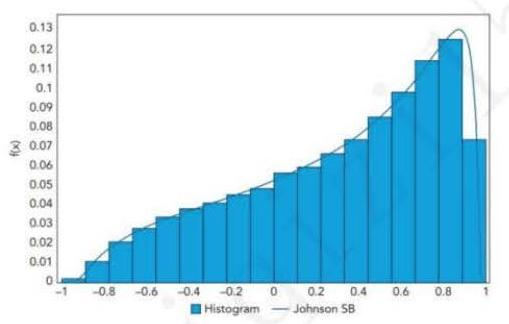
\includegraphics[width=0.4\textwidth]{images/01963dfb-ec81-7114-affc-d6d56ed48aa5_30_575_891_509_324_0.jpg}
\end{center}
\hspace*{3em} 


\subsection{金融相关性建模}


\begin{itemize}
    \item Copula functions are designed to simplify statistical problems. They allow the joining of multiple univariate distributions to a single multivariate distribution.
    \end{itemize}
    
    \begin{itemize}
    \item copula function:C 【公式不必记忆】
    \end{itemize}
    
    \[
    C\left\lbrack  {{G}_{1}\left( {u}_{1}\right) ，\ldots ，{G}_{n}\left( {u}_{n}\right) }\right\rbrack   = {F}_{n}\left\lbrack  {{F}_{1}^{-1}\left( {{G}_{1}\left( {u}_{1}\right) }\right) ，\ldots ，{F}_{n}^{-1}\left( {{G}_{n}\left( {u}_{n}\right) }\right) ;{\rho }_{F}}\right\rbrack
    \]
    
     \({\mathrm{G}}_{\mathrm{n}}\left( {\mathrm{u}}_{\mathrm{n}}\right)\) :边际分布 marginal distributions;
    
     \({\mathrm{F}}_{\mathrm{n}}\) : joint cumulative distribution function;
    
     \({\mathrm{F}}_{\mathrm{n}}^{-1}\left( {{\mathrm{G}}_{\mathrm{n}}\left( {\mathrm{u}}_{\mathrm{n}}\right) }\right.\) : the inverse of \({\mathrm{F}}_{\mathrm{n}}\) ;
    
     \({\rho }_{\mathrm{F}}\) : the correlation structure of \(\mathrm{{Fn}}\) 。
    
    \begin{itemize}
    \item Copulas became popular because they could presumably solve a complex problem in an easy way: it was assumed that copulas could correlate multiple assets;
    \end{itemize}
    
    \begin{itemize}
    \item for example， the 125 assets in a CDO， with a single， although multidimensional， function.
    \end{itemize}
    
    \begin{itemize}
    \item Gaussian (高斯) copula maps each unknown variable distribution (marginal distribution) to the standard normal distribution.
    \end{itemize}
    
     The rule for the mapping is percentile-to-percentile basis.
    
     Mapping a Gaussian Copula to the Standard Normal Distribution
    
    \begin{itemize}
    \item 重点理解这个原版书例题:
    \end{itemize}
    
    \begin{itemize}
    \item Let's assume we have two companies， B and Caa， with their estimated default probabilities for years 1 to 10 as displayed in Table.
    \end{itemize}
    
    \begin{center}
    \adjustbox{max width=\textwidth}{
    \begin{tabular}{|c|c|c|c|c|}
    \hline
    Default Time t & Company B Default Probability & Company B Cumulative Default Probability \({\mathrm{Q}}_{\mathrm{B}}\left( \mathrm{t}\right)\) & Company Caa Default Probability & Company Caa Cumulative Default Probability \({\mathrm{Q}}_{\mathrm{{Caa}}}\left( \mathrm{t}\right)\) \\
    \cline{1-5}
    1 & 6.51\% & 6.51\% & 23.83\% & 23.83\% \\
    \cline{1-5}
    2 & 7.65\% & 14.16\% & 13.29\% & 37.12\% \\
    \cline{1-5}
    3 & 6.87\% & 21.03\% & 10.31\% & 47.43\% \\
    \cline{1-5}
    4 & 6.01\% & 27.04\% & 7.62\% & 55.05\% \\
    \cline{1-5}
    5 & 5.27\% & 32.31\% & 5.04\% & 60.09\% \\
    \cline{1-5}
    6 & 4.42\% & 36.73\% & 5.13\% & 65.22\% \\
    \cline{1-5}
    7 & 4.24\% & 40.97\% & 4.04\% & 69.26\% \\
    \cline{1-5}
    8 & 3.36\% & 44.33\% & 4.62\% & 73.88\% \\
    \cline{1-5}
    9 & 2.84\% & 47.17\% & 2.62\% & 76.50\% \\
    \cline{1-5}
    10 & 2.84\% & 50.01\% & 2.04\% & 78.54\% \\
    \cline{1-5}
    \hline
    \end{tabular}
    }
    \end{center}
    
     具体而言:
    
    第一，已知违约概率，找到对应的累计违约概率。比如 B 公司两年内的累计违约 14.16\%=6.51\%+7.65\%。分别得出这两家公司的累计违约概率。
    
     第二步，映射。将表中的累积违约概率 \({\mathrm{Q}}_{\mathrm{B}}\left( \mathrm{t}\right)\) 、 \({\mathrm{Q}}_{\mathrm{{Caa}}}\left( \mathrm{t}\right)\) 分别映射到标准正态分布。比如，14.16\%映射到标准正态分布上的分位数是-1.0732。 year assuming a one-year Gaussian default correlation of 0.4 ?
    
    \begin{center}
    \adjustbox{max width=\textwidth}{
    \begin{tabular}{|c|c|c|c|c|}
    \hline
    Time t & Company B Cumulative Default Probability \({\mathrm{Q}}_{\mathrm{B}}\left( \mathrm{t}\right)\) & Company B Cumulative Standard Normal Percentiles \({\mathrm{N}}^{-1}\left( {{\mathrm{Q}}_{\mathrm{B}}\left( \mathrm{t}\right) }\right)\) & Company Caa Cumulative Default Probability Qcaa(t) & Company Caa Cumulative Standard Normal Percentiles \({\mathrm{N}}^{-1}\left( {{\mathrm{Q}}_{\mathrm{{Caa}}}\left( \mathrm{t}\right) }\right)\) \\
    \cline{1-5}
    1 & 6.51\% & -1.5133 & 23.83\% & -0.7118 \\
    \cline{1-5}
    2 & 14.16\% & -1.0732 & 37.12\% & -0.3287 \\
    \cline{1-5}
    3 & 21.03\% & -0.8054 & 47.43\% & -0.0645 \\
    \cline{1-5}
    4 & 27.04\% & -0.6116 & 55.05\% & 0.1269 \\
    \cline{1-5}
    5 & 32.31\% & -0.4590 & 60.09\% & 0.2557 \\
    \cline{1-5}
    6 & 36.73\% & -0.3390 & 65.22\% & 0.3913 \\
    \cline{1-5}
    7 & 40.97\% & -0.2283 & 69.26\% & 0.5032 \\
    \cline{1-5}
    8 & 44.33\% & -0.1426 & 73.88\% & 0.6397 \\
    \cline{1-5}
    9 & 47.17\% & -0.0710 & 76.50\% & 0.7225 \\
    \cline{1-5}
    10 & 50.01\% & 0.0003 & 78.54\% & 0.7906 \\
    \cline{1-5}
    \hline
    \end{tabular}
    }
    \end{center}
    
    \begin{itemize}
    \item what is the joint default probability \(\mathrm{Q}\) of companies \(\mathrm{B}\) and \(\mathrm{{Caa}}\) in the next
    \end{itemize}
    

    \[
    Q\left( {{t}_{b} \leq  1 \cap  {t}_{Caa} \leq  1}\right)
    \]
    
    \[
    \equiv  M\left( {{x}_{B} \leq   - {1.5133} \cap  {x}_{\text{ Caa }} \leq   - {0.7118}，\rho  = {0.4}}\right)  = {3.44}\%
    \]
    

    
    what is the joint probability of company \(\mathrm{B}\) defaulting in year 3 and company Caa defaulting in year 5 ?
    

    
    \[
    Q\left( {{t}_{B} \leq  3 \cap  {t}_{Caa} \leq  5}\right)
    \]
    
    \[
    \equiv  M\left( {{x}_{B} \leq   - {0.8054} \cap  {x}_{\text{ Caa }} \leq  {0.2557}，\rho  = {0.4}}\right)  = {16.93}\%
    \]
    
    
    
    Gaussian copula 中的违约相关性是 static correlation 静态相关性， 无法考虑动态相关性 dynamic correlation。
    
    【重点掌握， 给出表格会解读， 会找数据】
    












